\documentclass[12pt,a4paper]{article}

\usepackage[utf8]{inputenc}
\usepackage[T1]{fontenc}
\usepackage{polski}

\usepackage{amsthm}
\usepackage{amsmath}
\usepackage{amsfonts}
\usepackage{amssymb}
\usepackage{pgfplots}
\usepackage{tikz}
\usepackage{lmodern}	%fancy font
\usepackage{textcomp}

\usepackage{indentfirst}
\usepackage{graphicx}
\usepackage{caption}
\usepackage{subcaption}
\usepackage{siunitx}
\usepackage{here}


\setlength{\textheight}{24cm}
\setlength{\textwidth}{15.92cm}
\setlength{\footskip}{10mm}
\setlength{\oddsidemargin}{0mm}
\setlength{\evensidemargin}{0mm}
\setlength{\topmargin}{0mm}
\setlength{\headsep}{5mm}
\usepackage{tikz}
\usepackage{lmodern}	%fancy font
\usepackage{textcomp}

\usepackage{indentfirst}
\usepackage{graphicx}
\usepackage{caption}
\usepackage{subcaption}
\usepackage{siunitx}
\usepackage{here}
\usepackage[margin=1in]{geometry}% Just for this example
\setlength{\parindent}{0pt}% Just for this example
\setlength{\textheight}{24cm}
\setlength{\textwidth}{15.92cm}
\setlength{\footskip}{10mm}
\setlength{\oddsidemargin}{0mm}
\setlength{\evensidemargin}{0mm}
\setlength{\topmargin}{0mm}


\begin{document}

\begin{table}[H]
\label{my-label}
\begin{tabular}[width=\textwidth, height=0.5]{|c|p{11.0cm}|}
\hline
									           					&                           \\

\includegraphics[height=3cm]{img/logo}             					& \textbf{Technika cyfrowa} \\ \hline
\multicolumn{1}{|l|}{\textbf{Temat ćwiczenia}} 					& \textbf{Numer ćwiczenia}  \\
\multicolumn{1}{|l|}{Przerzutniki i rejestry}	& 3                         \\ \hline
\multicolumn{1}{|l|}{\textbf{Wykonawca}}       & \textbf{Ocena}            \\
\multicolumn{1}{|l|}{Michał Grabowski}          &                           \\ \hline
\end{tabular}
\end{table}

\section{Cel ćwiczenia}
Celem ćwiczenia numer 3 było zapoznanie się z różnymi rodzajami przerzutników (RS, JK, D) i zbudowanie z nich rejestrów SISO, SIPO, PIPO i PISO.

\section{Przebieg ćwiczenia}
\subsection{Asynchroniczny przerzutnik RS}
\subsubsection{Wykonanie}
\begin{figure}[H]
\centering
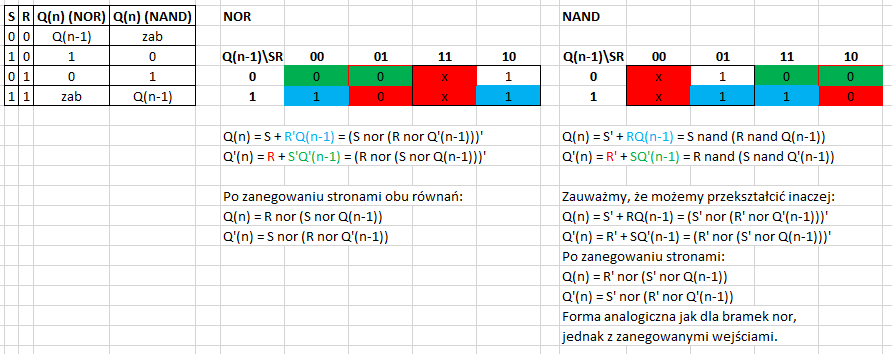
\includegraphics[width=\textwidth]{img/3a_karnaugh}
\end{figure}

Wykorzystując powyższą tabelę Karnaugh dla układu z bramek typu NOR, mamy następujące równania:
\begin{verse}
\centering
$Q(n) = S + \overline{R} \cdot Q(n-1) = \overline{(S \ nor \ (R \ nor \  \overline{Q(n-1)}))}$
\end{verse}
\begin{verse}
\centering
$\overline{Q(n)} = R + \overline{S} \cdot \overline{Q(n-1)}= \overline{(R \ nor \ (S \ nor \  Q(n-1))} $
\end{verse}
Negując teraz obie równości stronami, otrzymujemy oczekiwane rozwiązanie oparte o bramki NOR:
\begin{verse}
\centering
$Q(n) = R \ nor \ (S \ nor \ Q(n-1)) $ \\
\end{verse}
\begin{verse}
\centering
$\overline{Q(n)} = S \ nor \ (R \ nor \ \overline{Q(n-1)}$
\end{verse}

Wykorzystując powyższą tabelę Karnaugh dla układu z bramek typu NAND, mamy następujące równania, które przekształcając otrzymujemy rozwiązanie oparte o bramki NAND:
\begin{verse}
\centering
$Q(n) =  \overline{S} + R \cdot Q(n-1) = S \ nand \ (R \ nand \ Q(n-1))$
\end{verse}
\begin{verse}
\centering
$\overline{Q(n)} = \overline{R} + S \cdot \overline{Q(n-1)}  = R \ nand \ (S \ nand \ \overline{Q(n-1)}) $
\end{verse}

Zauważmy, że równości dla bramek NAND możemy przekształcić inaczej:
\begin{verse}
\centering
$Q(n) =  \overline{S} + R \cdot Q(n-1) = \overline{\overline{S} \ nor \ (\overline{R} \ nor \ \overline{Q(n-1))}}$
\end{verse}
\begin{verse}
\centering
$\overline{Q(n)} = \overline{R} + S \cdot \overline{Q(n-1)}  = \overline{\overline{R} \ nor \ (\overline{S} \ nor \ Q(n-1))} $
\end{verse}
Po zanegowaniu ich stronami otrzymujemy następujące wyniki:
\begin{verse}
\centering
$Q(n) = \overline{R} \ nor \ (\overline{S} \ nor \ Q(n-1)) $ \\
\end{verse}
\begin{verse}
\centering
$\overline{Q(n)} = \overline{S} \ nor \ (\overline{R} \ nor \ \overline{Q(n-1)})$
\end{verse}

Jak widać, zrealizowany na NANDach przerzutnik RS działa tak, jak gdybyśmy zanegowali wejścia S i R układu opartego o bramki NOR.

Na poniższym zrzucie ekranu przedstawiono działanie zaprojektowanego układu:

\begin{figure}[H]
\centering
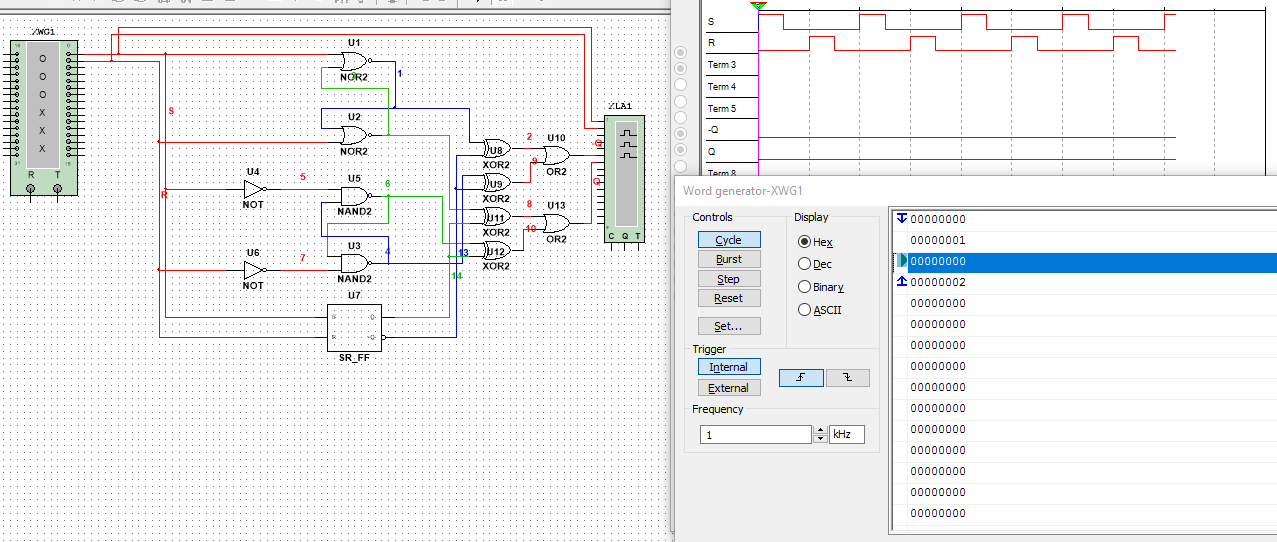
\includegraphics[width=\textwidth]{img/3a}
\end{figure}

\subsubsection{Wnioski}

Układ zachowuje się zgodnie z przewidywaniami (zastosowano bramki XOR, aby sprawdzić poprawność działania).

\subsection{Synchroniczny przerzutnik RS (reagujący na stan wysoki zegara)}
\subsubsection{Wykonanie}

Poniżej przedstawiono tabelę prawdy dla synchronicznego przerzutnika RS, który reaguje na stan wysoki zegara:

\begin{figure}[H]
\centering
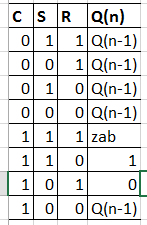
\includegraphics[scale=0.3]{img/3bTruthTable}
\end{figure}

W tym miejscu należy dokonać spostrzeżenia - zauważmy, że dla stanu zegarowego niskiego, przerzutnik na wyjściu ma poprzedni stan, natomiast dla stanu wysokiego, wyjście przerzutnika będzie identyczne z wyjściem zwykłego przerzutnika RS. Zatem układ synchronicznego przerzutnika RS reagującego na stan wysoki zegara, będzie składał się z asynchronicznego przerzutnika RS, którego wejścia będą odpowiednio wyjściami funkcji $S' \ = \ S \cdot C$ oraz $R' \ = \ R \cdot C$, ponieważ jeżeli sygnał zegarowy będzie niski - wówczas zarówno S' jak i R' będą 0, a więc podane do przerzutnika RS nie zmienią jego stanu, a w przeciwnym wypadku S' będzie równe S, a R' będzie równe R.

\begin{figure}[H]
\centering
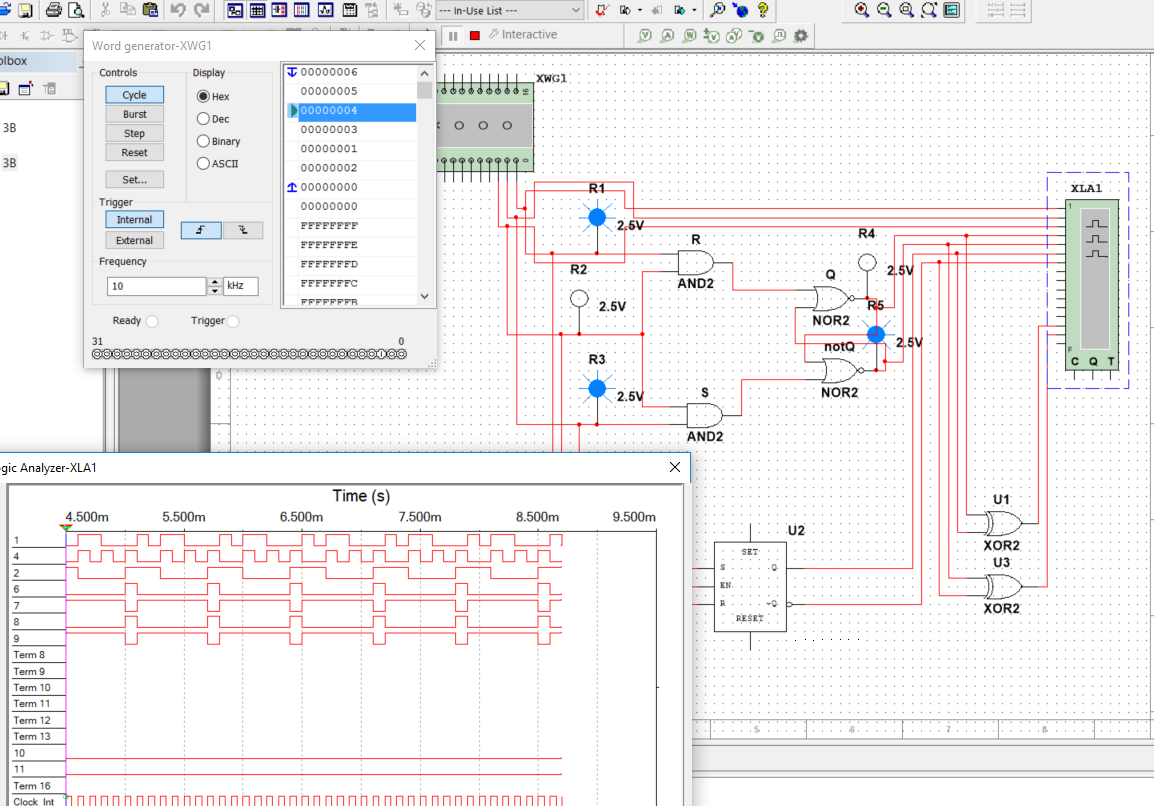
\includegraphics[width=\textwidth]{img/3b}
\end{figure}

\subsubsection{Wnioski}

Wnioski: Synchroniczny przerzutnik RS reaguje na wejścia R i S tylko, gdy wejście zegara jest w stanie wysokim. Z analizy logic analyzerem widać, iż zaprojektowany układ realizuje funkcję synchronicznego przerzutnika RS.
\\ 
Zastosowanie: synchroniczne przerzutniki RS są często stosowane przy taktowaniu sieci cyfrowych - dzięki temu można być pewnym, że ich elementy są ze sobą zsynchronizowane i skoordynowane.

\subsection{Synchroniczny przerzutnik JK}
\subsubsection{Wykonanie}
Poniżej przedstawiono tabelę prawdy dla synchronicznego przerzutnika JK:
\begin{figure}[H]
\centering
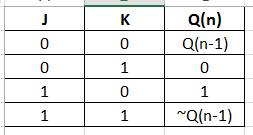
\includegraphics{img/3cTruthTable}
\end{figure}

Przerzutnik JK ma dwa wejścia:
\begin{itemize}
\item jedynkujące
\item kasujące
\end{itemize}
Jest on również synchroniczny. 

\begin{figure}[H]
\centering
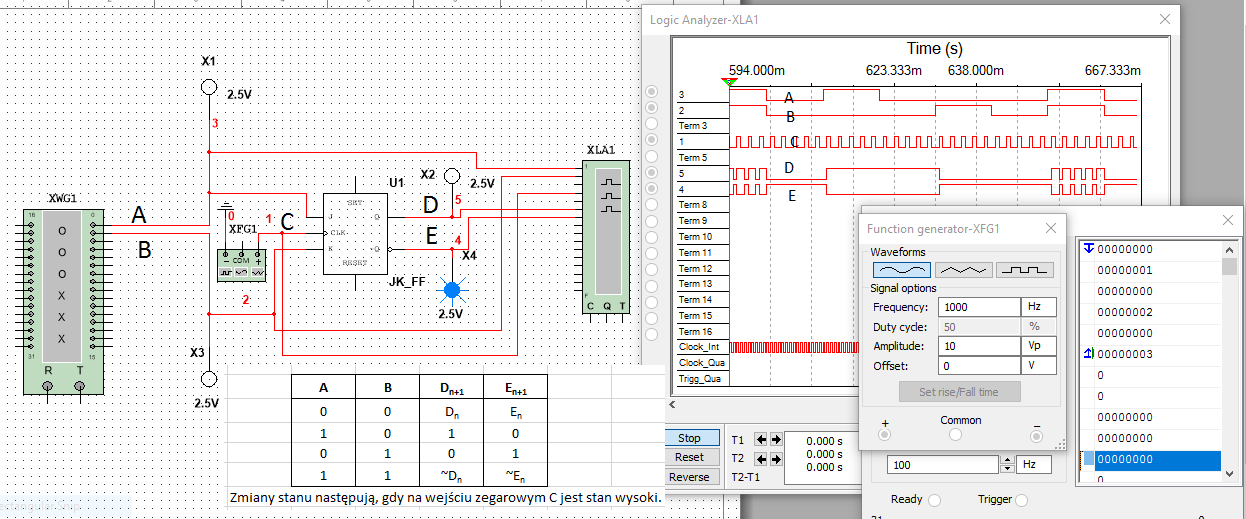
\includegraphics[width=\textwidth]{img/3c_syncJK}
\end{figure}

\subsubsection{Wnioski}

Wnioski: Jak widać na załączonym poniżej zrzucie ekranu, z sukcesem przetestowano działanie tego przerzutnika. \\
Ciekawostka: nazwa przerzutnika pochodzi od inicjałów  \textbf{Jacka Kilby'yego} - wynalazcy układu scalonego oraz laureata nagrody Nobla w dziedzinie fizyki (właśnie za wkład w wynalezienie układu scalonego).


\subsection{Przerzutnik D na podstawie asynchronicznego przerzutnika RS}
\subsubsection{Wykonanie}
Poniżej przedstawiono tabelę prawdy dla synchronicznego przerzutnika D:

\begin{figure}[H]
\centering
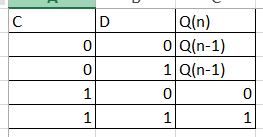
\includegraphics[width=0.3\textwidth]{img/3dTruthTable}
\end{figure}

Ponieważ przerzutnik D jest układem synchronicznym, to skorzystam z podobnego rozwiązania jak w realizacji synchronicznego przerzutnika RS - wykorzystam koniunkcje sygnału wejściowego i sygnału zegarowego, jednak tym razem, na podstawie tabeli prawdy, na wejście Reset podamy koniunkcję zanegowanego sygnału wejściowego i sygnału zegarowego, gdyż w przeciwnym wypadku na wyjściu otrzymalibyśmy poprzednie wyjście Q(n-1).

Skonstruowany układ przedstawiono na poniższym zrzucie ekranu:

\begin{figure}[H]
\centering
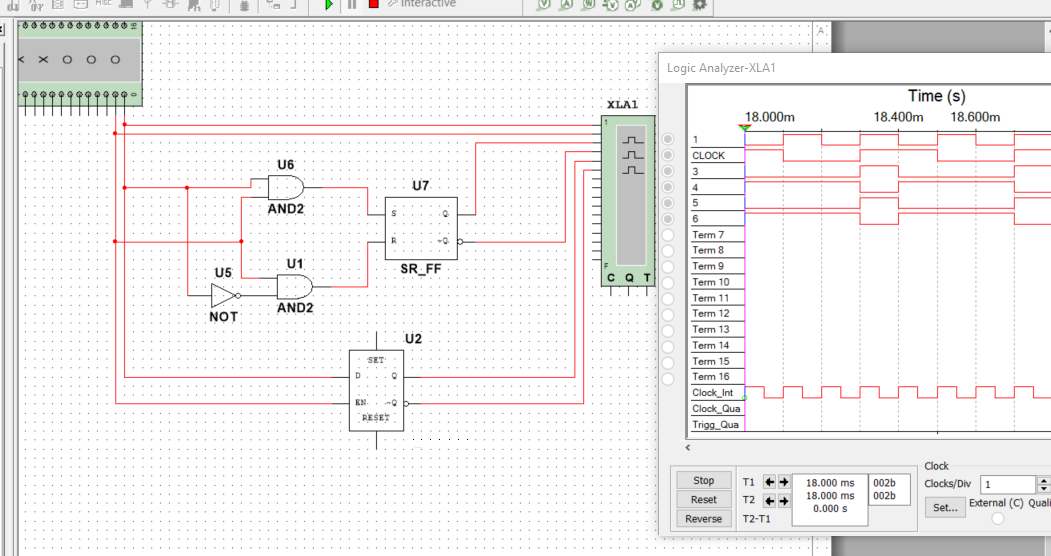
\includegraphics[width=\textwidth]{img/3d}
\end{figure}

\subsubsection{Wnioski}

Wnioski: Nazwa przerzutnika pochodzi z j. angielskiego - od słowa \textit{data} lub \textit{delay}. Jest to układ opóźniający - przepisuje sygnał wejściowy, ale tylko przy odpowiednim sygnale zegara. Jest to zatem także układ synchroniczny.
\\
Zastosowanie: Przerzutnik D znajduje szerokie zastosowanie w budowie rejestrów, jak pokazano w dalszych częściach ćwiczenia.	

\subsection{Przerzutnik T na podstawie synchronicznego przerzutnika D}
\subsubsection{Wykonanie}
Poniżej przedstawiono tabelę prawdy dla przerzutnika T:

\begin{figure}[H]
\centering
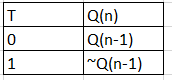
\includegraphics{img/3eTruthTable}
\end{figure}

Na poniższym zrzucie ekranu przedstawiono układ, który skonstruowano na podstawie analizy tabeli prawdy przerzutnika T oraz przerzutnika D:

\begin{figure}[H]
\centering
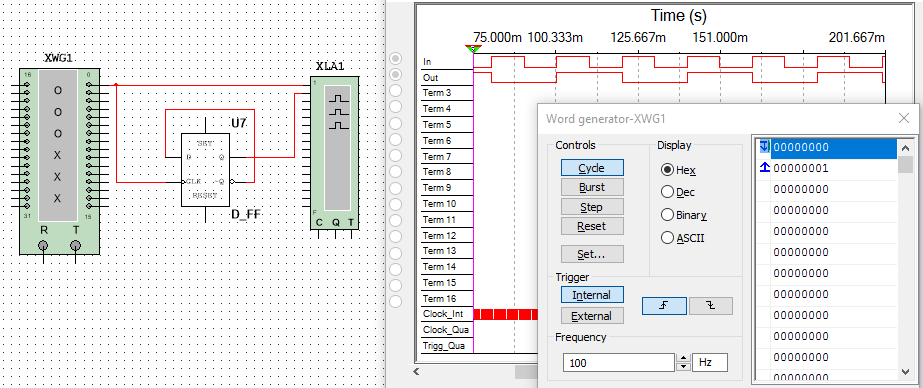
\includegraphics[width=\textwidth]{img/3e}
\end{figure}

\subsubsection{Wnioski}

Wnioski: Przerzutnik typu T (ang. \textit{Toggle}), który po podaniu stanu wysokiego na wejście T i opadnięciu sygnału zegarowego zmienia stan wyjścia na przeciwny od dotychczasowego.\\
Zastosowanie: znajduje zastosowanie w układach dzielenia częstotliwości przez 2.

\subsection{Przerzutnik D na podstawie synchronicznego przerzutnika JK}
\subsubsection{Wykonanie}
Poniżej przedstawiono tabelę prawdy dla synchronicznego przerzutnika D:
\begin{figure}[H]
\centering
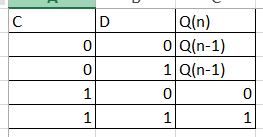
\includegraphics[width=0.3\textwidth]{img/3dTruthTable}
\end{figure}

Podobnie i tym razem, analizując tabele prawdy przerzutnika D oraz JK, skonstruowano i przetestowano obwód widoczny na poniższym zrzucie ekranu:

\begin{figure}[H]
\centering
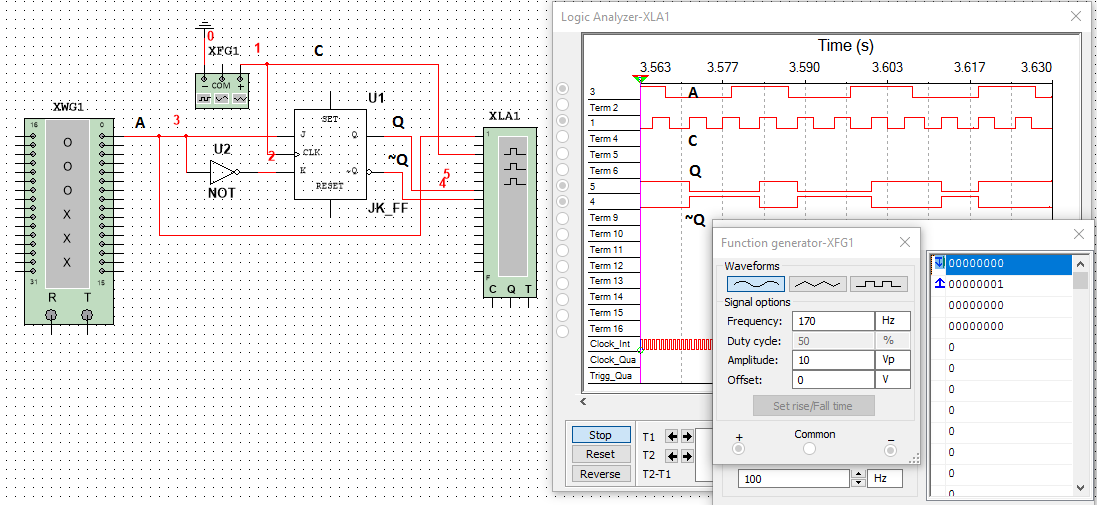
\includegraphics[width=\textwidth]{img/3f}
\end{figure}

\subsubsection{Wnioski}
Wnioski - na podstawie powyższych ćwiczeń można zauważyć, że w zależności od dostępnych elementów, przerzutnik D można zrealizować na wiele sposobów.


\subsection{Przerzutnik T na podstawie synchronicznego przerzutnika JK}
\subsubsection{Wykonanie}
Poniżej przedstawiono tabelę prawdy dla przerzutnika T:

\begin{figure}[H]
\centering
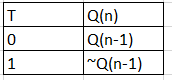
\includegraphics{img/3eTruthTable}
\end{figure}

Poniżej przedstawiono realizację zadanego układu oraz jego test:

\begin{figure}[H]
\centering
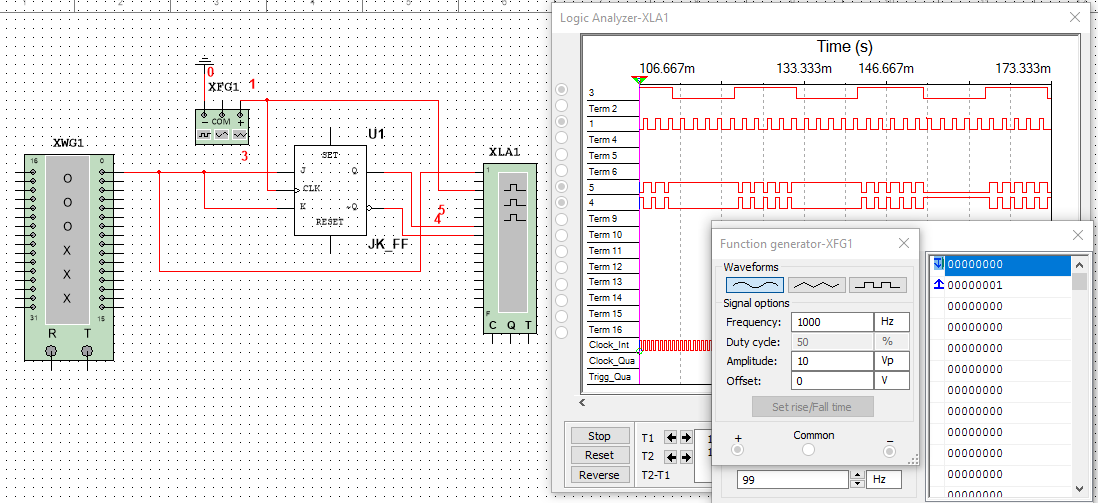
\includegraphics[width=\textwidth]{img/3g}
\end{figure}

\subsubsection{Wnioski}

Wnioski: Jak widać z powyższego i poprzedniego przykładu, prosty układ JK może być podstawą wielu przerzutników pełniących cały szereg różnych funkcji. 

\subsection{Rejestry na podstawie synchronicznych przerzutników D}

\subsubsection{Rejestr PIPO}
\begin{figure}[H]
\centering
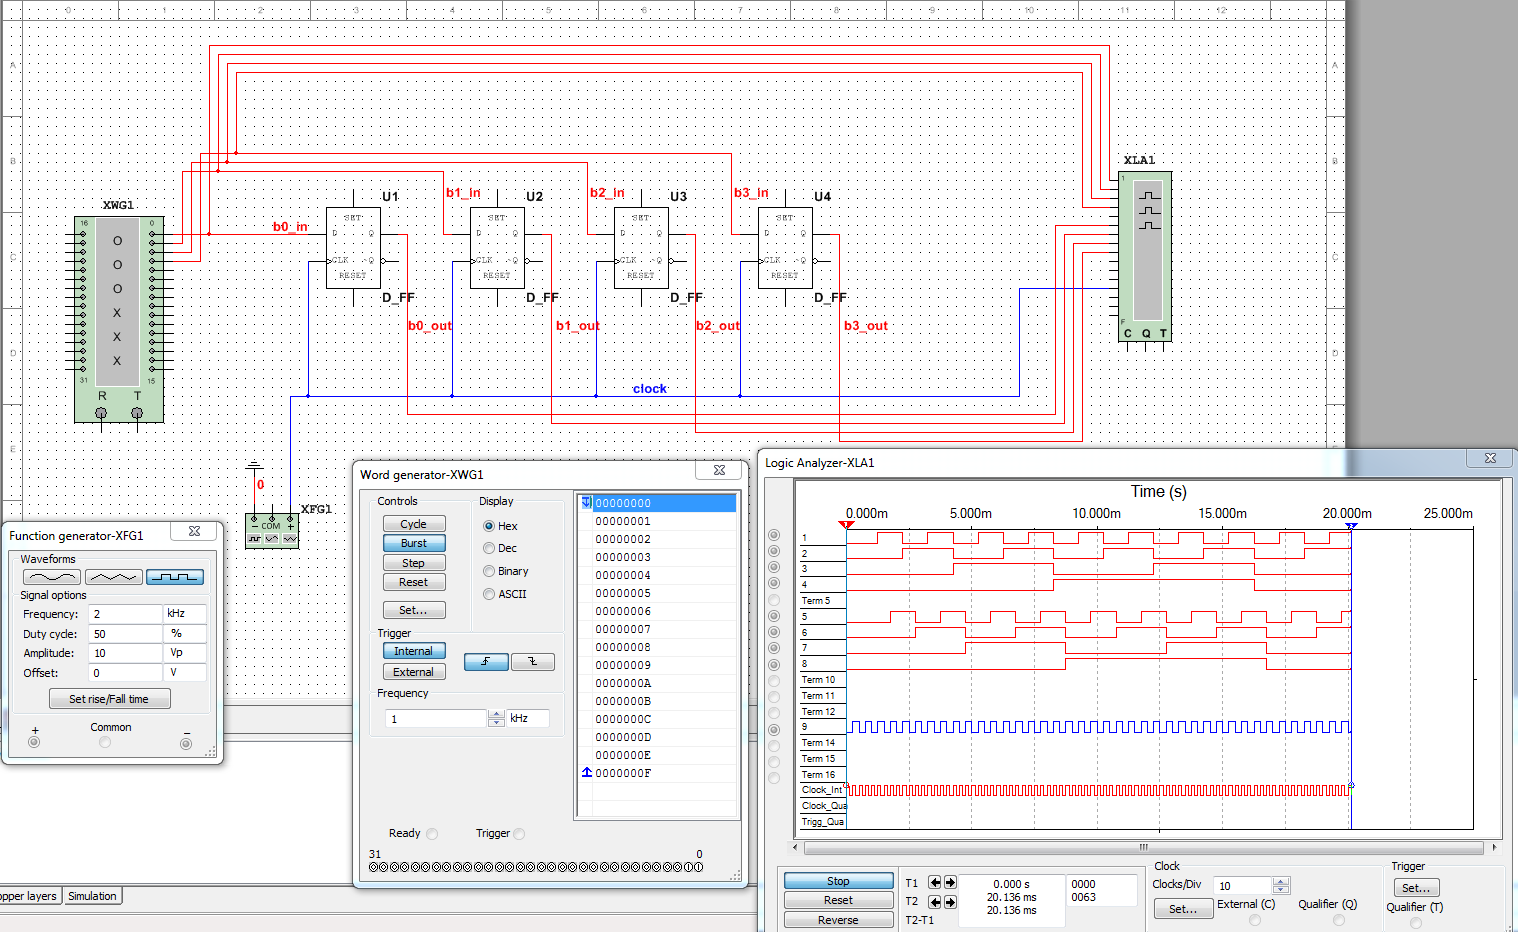
\includegraphics[width=\textwidth]{img/3hPIPO}
\end{figure}
\textbf{PIPO - Parallel-In Parallel-Out} - równoległe wejścia i równoległe wyjścia, czyli wejście i wyjście rejestru jest "szyną" 4 bitową - w każdym z przerzutników sygnał zmieniany jest tylko, gdy dany jest odpowiedni sygnał z zegara.

\subsubsection{Rejestr SIPO}
\begin{figure}[H]
\centering
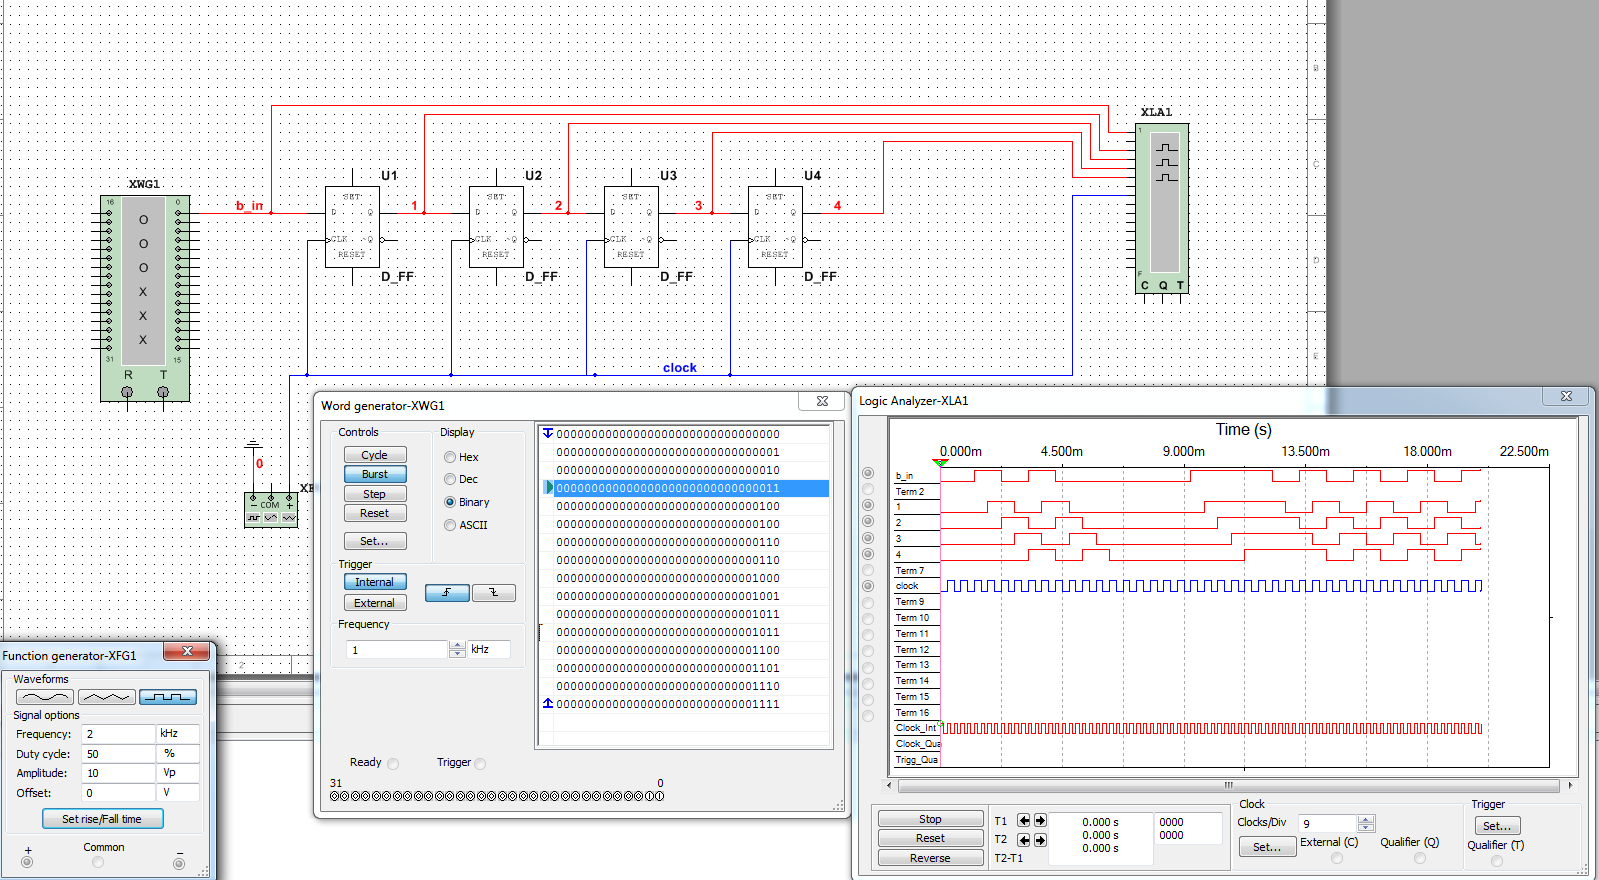
\includegraphics[width=\textwidth]{img/3hSIPO}
\end{figure}

\textbf{SIPO - Serial-In Parallel-Out} - szeregowe wejście, równoległe wyjście - na pojedynczym wejściu podajemy ciąg bitów, a na wyjściu dostajemy 4 równoległe bity. Wejście każdego kolejnego przerzutnika D podłączamy do wyjścia poprzedniego, wejście pierwszego z nich podłączamy do źródła danych. Wyjście każdego z przerzutników to kolejne bity wyjścia rejestru. Z każdym kolejnym cyklem zegara bity przesuwają się w prawo.
Bit najbardziej po prawej jest tracony, najbardziej po lewej jest odczytywany z wejścia szeregowego.

\subsubsection{Rejestr PISO}
\begin{figure}[H]
\centering
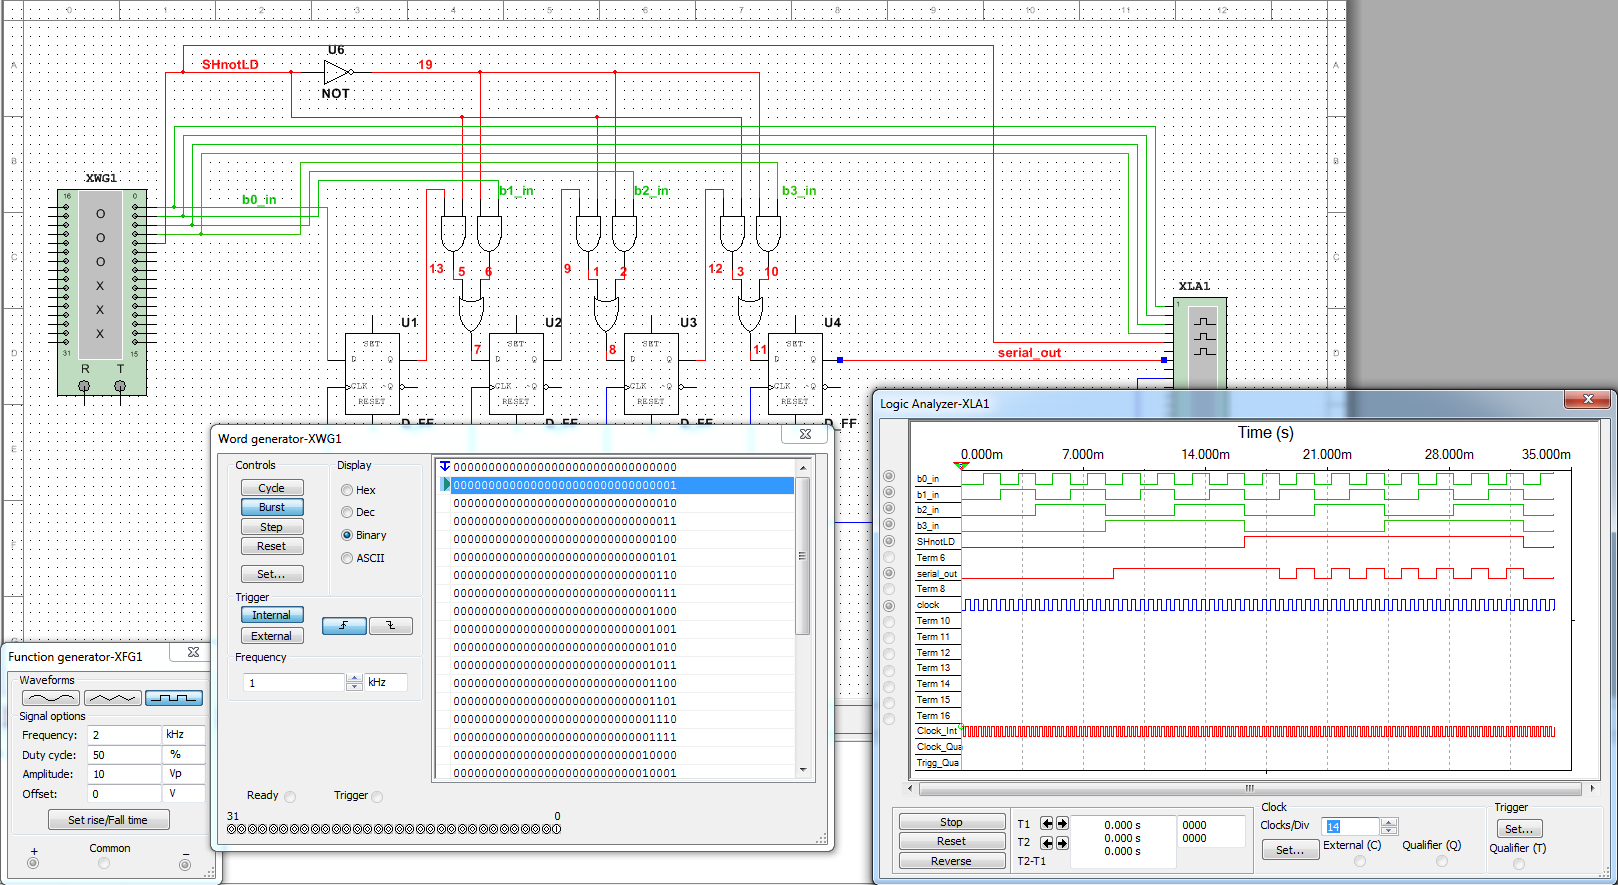
\includegraphics[width=\textwidth]{img/3hPISO}
\end{figure}

\textbf{PISO - Parallel-In Serial-Out} - na wejściu podajemy wiele sygnałów (równolegle), zaś na wyjściu otrzymujemy sygnał szeregowy. Potrzebna jest  możliwość wybrania - czy przesuwamy liczbę w rejestrze w prawo, czy też wczytujemy nową liczbę do rejestru wieloma wejściami. Osiąga się to następującą metodą:


Korzystamy z multipleksera - na wejściu dostaje on sterujący sygnał jednobitowy i dwa sygnały jednobitowe (źródła), między którymi będzie przełączał. W zależności od wartości sygnału sterującego, na wyjściu multipleksera pojawia się albo sygnał z jednego źródła, albo z drugiego. Na funkcji - jeżeli oznaczymy sygnał sterujący przez C, wejścia przez A, B, to multiplekser jednobitowy realizuje funkcję Y = AC + B(~C), czyli jeżeli C==1, na wyjściu jest A, jeżeli C==0, na wyjściu jest B.
W tym wypadku jednym ze źródeł jest wyjście poprzedniego rejestru (bo chcemy móc przesuwać bity w rejestrze), a drugim jest wejście danych (czyli miejsce, skąd chcemy wpisać dane do rejestru). 
Do każdego wejścia równoległego oprócz pierwszego dodajemy taki multiplekser. Sygnałem sterującym jest SHnotLD - jeżeli sygnał sterujący jest wysoki to wykonujemy SHift - przesunięcie, a jeżeli jest niski, to wykonujemy LoaD - załadowanie nowej liczby do rejestru.

\subsubsection{Rejestr SISO}
\begin{figure}[H]
\centering
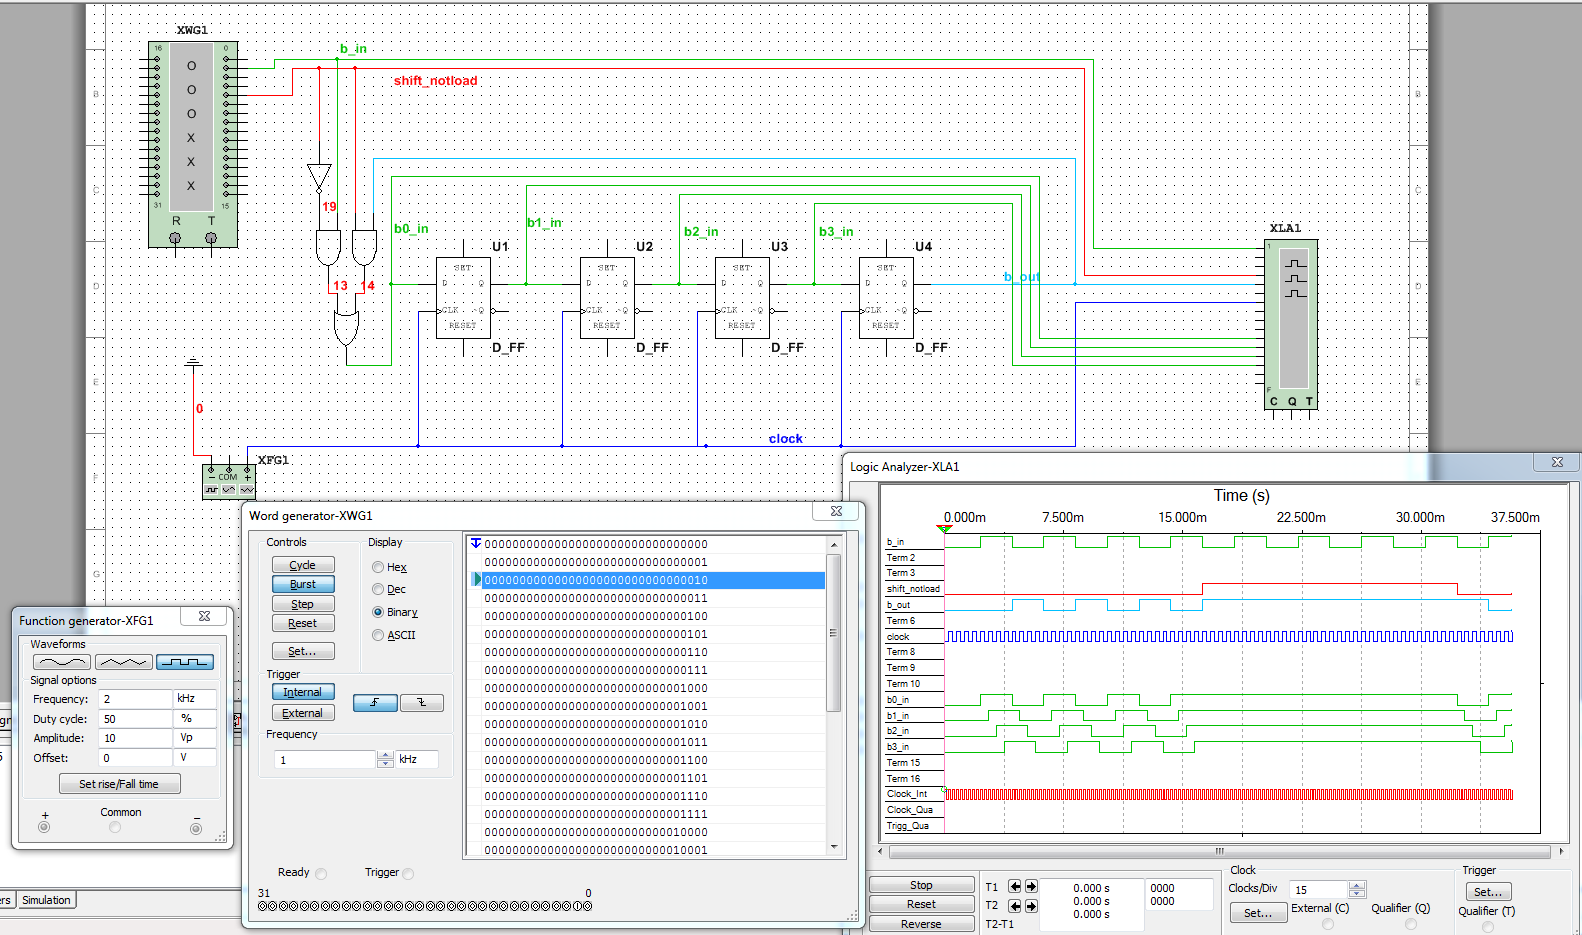
\includegraphics[width=\textwidth]{img/3hSISO}
\end{figure}

\textbf{SISO - Serial-In Serial-Out} - ten rejestr szeregowo dostaje dane i szeregowo ma je zwrócić. Ponieważ na wejściu dostajemy cały czas jakiś sygnał, to chcemy zapobiec utracie to, co w rejestrze jest. Dlatego tutaj też stosujemy multiplekser korzystający z sygnału SHnotLD, tym razem jednak używamy go, żeby "zapętlić" wyjście szeregowe z wejściem. Wtedy sygnałem SHnotLD, wybieramy czy przesuwamy dalej dane w prawo gubiąc stare (dla sygnału 1 SHnotLD), czy też zapętlamy wyjście z wejściem, czyli efektywnie to co było w rejestrze, będzie się w nim zapętlać.

\subsubsection{Rejestry - wnioski}
Można zauważyć, że korzystające z transmisji szeregowej (bardzo często stosowanej współcześnie w elektronice, np. w USB, Ethernet) rejestry obarczone są opóźnieniem w działaniu, wynikającym nie tylko z częstotliwości taktowania wejścia zegarowego, ale także samej konstrukcji - ponieważ składają się one z przerzutników D, z których każdy posiada pewne opóźnienie w działaniu, związane z opóźnieniem bramek logicznych, na których go zbudowano. Opóźnienie to się zwielokrotnia, bo aby załadować dane do rejestru SIPO/SISO lub odczytać dane z rejestru PISO/SISO należy wykonać odpowiednią liczbę przesunięć w rejestrze.

W związku z powyższym, teoretycznie najszybszy w działaniu powinien być rejestr PIPO, jednak wymaga on odpowiednich 'szyn' na dane.

\end{document}
